A Support Vector Machine(SVM) is a classifier which outputs an optimal hyperplane or set of hyperplanes in high-dimensional space and classifies data. A hyperplane in an n-dimensional space, is a subspace of one dimension less than the whole space. In figure \ref{fig:SVM} a hyperplane of 2-dimensional space is a line which divides the 2-dimensional space in half. This division defines two closed half-space, and represents the division between two classes. The original idea for SVM was conceived by Cortes and Vapnik in 1995 \cite{cortes1995support} \\
In figure \ref{fig:SVM} main idea behind SVM is shown. Consider example dataset described by variables $x_1$ and $x_2$ and suppose we want to classify all the elements(elements are shown by class circle and class square). The operation of SVM algorithm is based on finding the optimal hyperplane between the two classes \cite{opencv_library}. An optimal hyperplane is one that gives the largest minimum distance to the classes and it maximizes the margin between the hyperplane and all data points. %i.e. the best line that leaves the maximum margin from both classes.

\begin{figure}[H]
    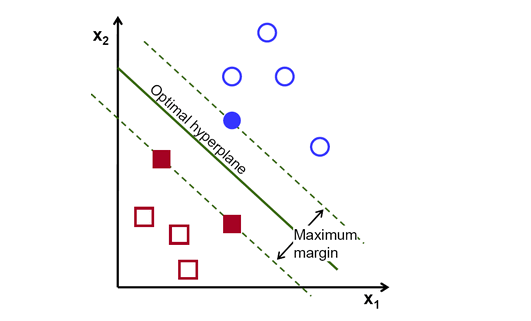
\includegraphics[width=0.45\textwidth]{./img/SVM.png}
     \caption{\footnotesize{SVM for separable binary set}}
    \label{fig:SVM}
\end{figure}

%Klopt dit stuk? Heeft SVM geen last van curse of dimensionality? If so, misschien wat meer uitleg. Sowieso meer uitleg over de karakteristieken van SVM zou nice zijn. Dat kan goed gequote worden in de latere discussie.
SVM are popular for couple of theoretical reasons: SVMs are robust to very large number of variables and can learn both simple and complex classification models \cite{cristianini2000}.\\

%Ik snap niks van dit stuk, kan hier meer uitleg over?
SVMs is a best known member in the general category of kernel methods \cite{shawe2004kernel}. A kernel method has the ability to generate non-linear decision boundaries by using method designed for linear classifiers. It turns out SVM does not need to work on higher-dimensional space implicitly because a kernel method rely on data through dot-products. Dot product can be replaced by kernel function which compute dot product in higher dimensional space. This allows the user to apply a classifier to data that has infinite- dimensional vector space representation such as DNA or protein \cite{ben2010user}.\\
%Dank je :D

In recent years, SVMs are widely used in bio-informatics \cite{furey2000support,osuna1997training,guyon2002gene} and other disciplines due to its ability to accurately deal with high dimensional data\cite{joachims1998text}. In marine environments, researchers have proposed a method for detection of oil spills in SAR images, using SVM  as a classifier. 
%Heeft SVM extra veel last van noise?? Volgens mij kan elke classifier wel baat hebben bij noise reduction....
The result of this research has shown that SVM has better performance on SAR image when using texture analysis and decomposition algorithm in various steps of the SVM algorithm. Texture analysis will help to reduce noise in SAR image \cite{matkan2013oil}.
